
% \documentclass[draft,11pt]{article}
\chapter{Random Matrix Concentration and Spectral Graph
  Sparsification}
\label{cha:randmat}
%\usepackage{cleveref}

%\allowdisplaybreaks

%%% for this lecture
%\newcommand\symset{S}
%\newcommand\psdset{S_+}
%\newcommand\pdset{S_{++}}

%\newcommand\symsetn{\symset^n}
%\newcommand\psdsetn{\psdset^n}
%\newcommand\pdsetn{\pdset^n}

%%% added by Hongjie
%\newcommand{\Hongjie}[1]{{\color{red} Hongjie: #1}}


%\begin{document}
\sloppy
%\lecture{8 --- Wednesday, April 8th}
%{Spring 2020}{Rasmus Kyng, Scribe: Hongjie Chen}{Random Matrix
%Concentration and Spectral Graph Sparsification}



\section{Matrix Sampling and Approximation}

We want to begin understanding how sums of random matrices behave, in
particular, whether they exhibit a tendency to concentrate in the same
way that sum of scalar random variables do under various conditions.

First, let's recall a scalar Chernoff bound, which shows that a sum of
bounded, non-negative random variables tend to concentrate around
their mean.
\begin{theorem}[A Chernoff Concentration Bound]
Suppose $X_1, \ldots, X_k \in \R$ are independent, non-negative,
random variables with $X_i \leq R$ always.
Let $X = \sum_i X_i$, and $\mu = \E{X}$,
then for $0 < \epsilon \leq 1$
\[
\Pr[ X \geq (1+\epsilon) \mu ] \leq \exp\left(\frac{-\epsilon^2
    \mu}{4R}\right)
\text{ and }
\Pr[ X \leq (1-\epsilon) \mu] \leq \exp\left(\frac{-\epsilon^2
    \mu}{4R}\right)
.
  \]
\end{theorem}
The Chernoff bound should be familiar to most of you, but you may not
have seen the following very similar bound.
The Bernstein bound, which we will state in terms of zero-mean
variables, is much like the Chernoff bound.
It also requires bounded variables.
But, when the variables have small variance, the Bernstein bound is
sometimes stronger.
\begin{theorem}[A Bernstein Concentration Bound]
  \label{thm:bernstein}
  Suppose $X_1, \ldots, X_k \in \R$ are independent, zero-mean,
random variables with $\abs{X_i} \leq R$ always.
Let $X = \sum_i X_i$, and $\sigma^2 = \Var{X} = \sum_i \E{X_i^2}$,
then for $\epsilon > 0$
\[
\Pr[ \abs{X} \geq t] \leq 2\exp\left(\frac{-t^2}{2Rt +
    4\sigma^2}\right)
.
  \]
\end{theorem}
We will now prove the Bernstein concentration bound for scalar random
variables, as a warm-up to the next section, where we will prove a version
of it for matrix-valued random variables.
To help us prove Bernstein's bound, first let's recall Markov's
inequality.
This is a very weak concentration inequality, but also very versatile,
because it requires few assumptions.
\begin{lemma}[Markov's Inequality]
  \label{lem:markov}
  Suppose $\XX \in \R$ is a non-negative random variable, with a finite
  expectation.
  Then for any $t > 0$,
  \[
    \Pr[ X \geq t] \leq \frac{\E{X}}{t}
    .
    \]
\end{lemma}
\begin{proof}
  \begin{align*}
    \E{X}
    &=
      \Pr[X \geq t]\E{X \mid X \geq t} + \Pr[X < t]\E{X \mid X < t}
   \\
    &\geq \Pr[X \geq t]\E{X \mid X \geq t}
    \\
    &\geq Pr[X \geq t] \cdot t
      .
\end{align*}
  We can rearrange this to get the desired statment.
\end{proof}
Now, we are ready to prove Bernstein's bound.
\begin{proof}[Proof of Theorem~\ref{thm:bernstein}]
  We will focus on bounding the probability that $\Pr[ X \geq t] $.
  The proof that $\Pr[ -X \geq t] $ is small proceeds in the same way.

  First we observe that
  \begin{align*}
    \Pr[ X \geq t ]
    &=
      \Pr [ \exp(\theta X) \geq \exp(\theta t) ]
      \tag*{for any $\theta >0$,
      because $x \to \exp(\theta x)$ is strictly increasing.}
    \\
    &\leq \exp(-\theta t) \E{\exp(\theta X)}
      \tag*{by Lemma~\ref{lem:markov} (Markov's Inequality).}
  \end{align*}
  Now, let's require that $\theta \leq 1/R$
  This will allow us to using the following bound: For all $\abs{z}
  \leq 1$,
  \begin{equation}
     \label{eq:expub}
  \exp(z) \leq 1+z+z^2.
\end{equation}
We omit a proof of this, but the plots in Figure~\ref{fig:expub}
suggest that this upper bound holds. The reader should consider how to
prove this.
\begin{figure}[h]
  \centering
  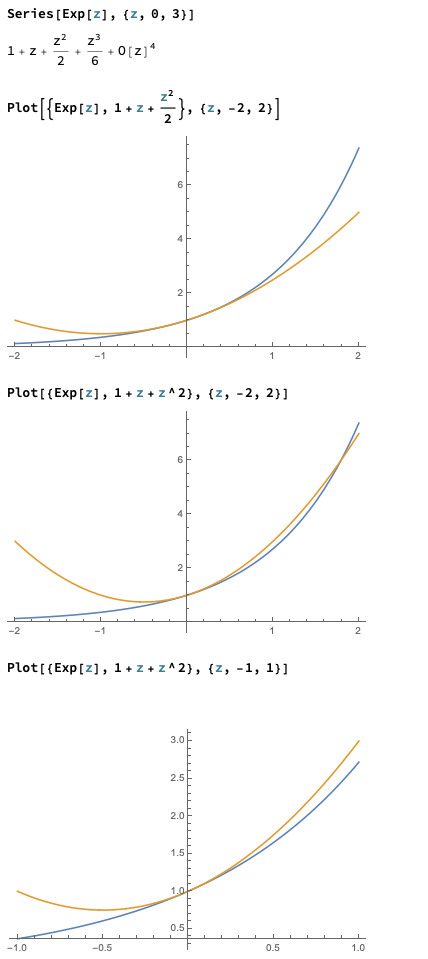
\includegraphics[width=0.4
  \textwidth]{fig/lecture7_exp-bounds}
\caption{Plotting $\exp(z)$ compared to $1+z+z^2$.}
\label{fig:expub}
\end{figure}
With this in mind, we see that
\begin{align*}
  \E{\exp(\theta X)}
  &= \E{\exp\left(\theta \sum_i X_i\right)}
  \\
  &=\E{\Pi_{i} \exp(\theta X_i)}
  \\
  &=\Pi_{i} \E{\exp{(\theta X_i)}}
    \tag*{because $\E{YZ} = \E{Y}\E{Z}$ for independent $Y$ and
    $Z$.} % See note\footnote{ hello }}%\todo{text}}.
  \\
  &\leq\Pi_{i} \E{1+\theta X_i+(\theta X_i)^2}
  \\
  &=\Pi_{i} (1+\theta^2\E{ X_i^2})
  \\
  &\leq\Pi_{i} \exp( \theta^2\E{ X_i^2} )
    \tag*{ because $1+z \leq \exp(z)$ for all $z \in R$.}
  \\
  &=\exp\left( \sum_i \theta^2\E{ X_i^2} \right) = \exp(\theta^2 \sigma^2)
    .
\end{align*}
Thus
$\Pr[ X \geq t ] \leq \exp(-\theta t)\E{\exp(\theta X)} \leq
\exp(-\theta t + \theta^2 \sigma^2)$.
Now, to get the best possible bound, we'd like to minimize
$-\theta t + \theta^2 \sigma^2$ subject to the constraint
$0< \theta \leq 1/R$.
Setting
\[ \frac{\partial}{\partial \theta}\left(
    -\theta t + \theta^2
    \sigma^2
  \right)
  = - t + 2 \theta \sigma^2
  .
\]
Setting this derivative to zero gives
$\theta = \frac{t}{2\sigma^2}$,
and plugging that in gives
\[
    -\theta t + \theta^2\sigma^2
    =
    -\frac{t^2}{4\sigma^2}
  \]
This choice only satisfies our constraints on $\theta$ if
$\frac{t}{2\sigma^2} \leq 1/R$.
Otherwise, we let $\theta =  1/R$ and note that in this case
\[
    -\theta t + \theta^2\sigma^2
    =
    -\frac{t}{R} + \frac{\sigma^2}{R^2}
    \leq
    -\frac{t}{R} + \frac{t}{2R}
    =
    -\frac{t}{2R}
  \]
  where we got the inequality from $t > 2\sigma^2/R$.
  Altogether, we can conclude that there always is a choice of
  $\theta$ s.t.
  \[
    -\theta t + \theta^2\sigma^2
    \leq
    - \min\left( \frac{t}{2R} , \frac{t^2}{4\sigma^2} \right)
    \leq
    - \frac{t^2}{2Rt + 4\sigma^2}
    .
  \]
  In fact, with the benefit of hindsight, and a little algebra, we
  arrive at the same conclusion in another way:
  One
  can check that the
  following choice of $\theta$ is always valid and achives the same
  bound:
  $\theta = \frac{1}{2
    \sigma^2}\left( t - \frac{\sqrt{R} \cdot t^{3/2}}{\sqrt{2\sigma^2 + R
        t}} \right)$.
\end{proof}
We use $\norm{\cdot}$ to denote the spectral norm on matrices.
Let's take a look at a version of Bernstein's bound that applies to
sums of random matrices.
\begin{theorem}[A Bernstein Matrix Concentration Bound (Tropp 2011)]
  \label{thm:matbernstein}
  Suppose $\XX_1, \ldots, \XX_k \in \R^{n \times n}$ are independent,
  symmetric matrix-valued
  random variables.
Assume each $\XX_i$ is zero-mean, i.e. $\E{\XX_i} = \matzero_{n \times
  n}$, and that $\norm{\XX_i} \leq R$ always.
Let $\XX = \sum_i \XX_i$, and $\sigma^2 = \norm{\Var{\XX}} = \norm{\sum_i \E{\XX_i^2}}$,
then for $\epsilon > 0$
\[
\Pr[ \norm{\XX} \geq t] \leq 2n\exp\left(\frac{-t^2}{2Rt + 4\sigma^2}\right)
.
\]
\end{theorem}
This basically says that probability of $\XX$ being large in spectral
norm behaves like the scalar case, except the bound is larger by a factor
$n$, where the matrices are $n \times n$.
We can get a feeling for why this might be a reasonable bound by
considering the case of random diagonal matrices.
Now $\norm{\XX} = \max_j \abs{\XX (j,j)} = \max_j \abs{\sum_i
  \XX_i(j,j)}$.
In this case, we need to bound the largest of the $n$ diagonal
entries: We can do this by a union bound over $n$ instances of the
scalar problem -- and this also turns out to be essentially tight in some cases,
meaning we can't expect a better bound in general.

\section{Matrix Concentration}
In this section we will prove the Bernstein matrix concentration bound
(Tropp 2011) that we saw in the previous section.
\begin{theorem}\label{thm:matbernstein}
  Suppose $\XX_1, \ldots, \XX_k \in \R^{n \times n}$ are independent, symmetric matrix-valued random variables.
  Assume each $\XX_i$ is zero-mean, i.e. $\E{\XX_i} = \matzero_{n \times
  n}$, and that $\norm{\XX_i} \leq R$ always.
  Let $\XX = \sum_i \XX_i$, and $\sigma^2 = \|\Var{\XX}\| = \|\sum_i \E{\XX_i^2}\|$, then for $t > 0$
  \[
  \Pr[ \norm{\XX} \geq t] \leq 2n\exp\left(\frac{-t^2}{2Rt + 4\sigma^2}\right).
  \]
\end{theorem}
But let's collect some useful tools for the proof first.

\begin{definition}[trace]
  The trace of a square matrix $\AA$ is defined as
  \[ \trace{\AA} := \sum_{i} \AA(i,i) \]
\end{definition}

\begin{claim}[cyclic property of trace]
  $\trace{\AA\BB} = \trace{\BB\AA}$
\end{claim}

Let $S^n$ denote the set of all $n\times n$ real symmetric matrices,
$S^n_+$ the set of all $n\times n$ positive semidefinite matrices,
and $S^n_{++}$ the set of all $n\times n$ positive definite matrices.
Their relation is clear, $S^n_{++} \subset S^n_+ \subset S^n$.
For any $\AA\in S^n$ with eigenvalues $\lambda_1(\AA)\leq\cdots\leq\lambda_n(\AA)$, by spectral decomposition theorem, $\AA = \VV\LLambda\VV^\trp$ where $\LLambda=\diag_i\{\lambda_i(\AA)\}$ and $\VV^\trp\VV=\VV\VV^\trp=\II$,
we'll use this property without specifying in the sequel.

\begin{claim}\label{clm:tr_eq_sum_eigen}
  Given a symmetric and real matrix $\AA$, $\trace{\AA} = \sum_{i}\lambda_i$, where $\{\lambda_i\}$ are eigenvalues of $A$.
\end{claim}
\begin{proof}
  \[ \trace{\AA} = \trace{\VV\LLambda\VV^\trp} = \trace{\LLambda\underbrace{\VV^\trp\VV}_{\II}} = \trace{\LLambda} = \sum_i \lambda_i. \]
\end{proof}

\subsection{Matrix Functions}
\begin{definition}[Matrix function]
  Given a real-valued function $f:\R\to\R$, we extend it to a matrix function $f:S^n\to S^n$.
  For $\AA\in S^n$ with spectral decomposition $\AA=\VV\LLambda\VV^\trp$, let
  \[ f(\AA) = \VV \diag_i\left\{f(\lambda_i)\right\} \VV^\trp. \]
\end{definition}
\begin{example}
  Recall that every PSD matrix $\AA$ has a square root $\AA^{1/2}$.
  If $f(x) = x^{1/2}$ for $x\in\R_+$, then $f(\AA)=\AA^{1/2}$ for $\AA\in S^n_+$.
\end{example}
\begin{example}
  If $f(x) = \exp(x)$ for $x\in\R$, then $f(\AA) = \exp(\AA) = \VV\exp(\LLambda)\VV^\trp$ for $\AA\in S^n$.
  Note that $\exp(\AA)$ is positive definite for any $\AA\in S^n$.
\end{example}

\subsection{Monotonicity and Operator Monotonicity}
 Cosider a function $f:
 \calD \to \calC$.
 If we have a partial order $\leq_{\calD}$ defined on $\calD$ and a
 partial order $\leq_{\calC}$ defined on $\calC$, then we say that
 the function is monotone increasing (resp. decreasing) w.r.t. this pair of orderings if for all $d_1, d_2
 \in \calD$ s.t. $d_1 \leq_{\calD} d_2$ we have $f(d_1) \leq_{\calC}
 f(d_2) $ (resp. decreasing if $f(d_2) \leq_{\calC} f(d_1)$).

Let's  introduce some terminonology for important special cases of this idea.
We say that a function $f : \calS \to \R$, where $\calS \subseteq \symsetn$,
  is monotone increasing if $\AA \preceq \BB$ implies $f(\AA) \leq f(\BB)$.

  Meanwhile, a function $f : \calS \to \calT$ where $\calS, \calT \subseteq \symsetn$
  is said to be operator monotone increasing if $\AA \preceq \BB $ implies
  $f(\AA) \preceq f(\BB)$.
%
\begin{lemma}
  Let $T \subseteq \R$.
  If the scalar function $f : T \to \R$ is monotone increasing, the matrix
  function $\XX \mapsto \trace{f(\XX)}$ is monotone increasing.
\end{lemma}
\begin{proof}
  From previous chapters, we know if $\AA\preceq\BB$ then $\lambda_i(\AA)\leq\lambda_i(B)$ for all $i$.
  As $x \mapsto f(x)$ is monotone, then $\lambda_i(f(\AA))\leq\lambda_i(f(B))$ for all $i$.
  By Claim \ref{clm:tr_eq_sum_eigen}, $\trace{f(\AA)}\leq\trace{f(\BB)}$.
\end{proof}
From this, and the fact that $x \mapsto \exp(x)$ is a monotone function on the
reals, we get the following corollary.
\begin{corollary}\label{cor:trexpmono}
  If $\AA\preceq\BB$, then $\trace{\exp(\AA)}\leq\trace{\exp(\BB)}$,
  i.e. $\XX \mapsto \trace{\exp(\XX)}$ is monotone increasing.
\end{corollary}

\begin{lemma}\label{lem:invmono}
  If $\matzero \prec\AA\preceq\BB$, then $\BB^{-1}\preceq \AA^{-1}$, i.e. $\XX
  \mapsto \XX^{-1}$ is operator monotone decreasing on $\pdsetn$.
\end{lemma}
You will prove the above lemma in this week's exercises.

\begin{lemma}\label{lem:logmono}
  If $0\prec\AA\preceq\BB$, then $\log(\AA)\preceq\log(\BB)$.
\end{lemma}
To prove this lemma, we first recall an integral representation of the
logarithm.
\begin{lemma}
  \label{lem:logintegral}
\[
\log a = \int_0^{\infty} \left(\frac{1}{1+t} -\frac{1}{a+t}  \right)
\diff t
    \]
\end{lemma}
\begin{proof}
  \begin{align*}
\int_0^{\infty} \left(\frac{1}{1+t} -\frac{1}{a+t}  \right) \diff t
    &=
    \lim_{T \to \infty}
      \int_0^{T} \left(\frac{1}{1+t} -\frac{1}{a+t}  \right) \diff t
\\
    &=
    \lim_{T \to \infty}
      \left[ \log(1+t) - \log(a+t) \right]_0^{T}
\\
    &=
      \log(a)
      +
    \lim_{T \to \infty}
      \log\left( \frac{1+T}{a+T} \right)
\\
    &=
      \log(a)
  \end{align*}
\end{proof}
\begin{proof}[Proof sketch of Lemma~\ref{lem:logmono}]
Because all the matrices involved are diagonalized by the same
orthogonal transformation, we can conclude from
Lemma~\ref{lem:logintegral} that for a matrix $\AA \succ \matzero$,
\[
 \log(\AA)
   = \int_0^{\infty} \left(\frac{1}{1+t}\II -(t \II + \AA)^{-1} \right) \diff t
\]
This integration can be expressesd as the limit of a sum with positive
coefficients, and from this we
can show that is the integrand (the term inside the integration
symbol) is operator monotone increasing in $\AA$ by
Lemma~\ref{lem:invmono}, the result of the integral, i.e. $\log(\AA)$
must also be operator monotone increasing.
\end{proof}

The following is a more general version of Lemma 1.6.
\begin{lemma}
  Let $T \subset \R$.
  If the scalar function $f : T \to \R$ is monotone, the matrix
  function $\XX \mapsto \trace{f(\XX)}$ is monotone.
\end{lemma}

\begin{remark}
  It is not always true that when $f: \R \to \R$ is monotone, $f:
  \symsetn \to \symsetn$ is operator monotone.
  For example, $\XX \mapsto \XX^2$ and $\XX \mapsto \exp(\XX)$ are \emph{not}
  operator monotone.
  % while ${\XX \to (\XX)^{1/2}}$ is operator monotone
  % over $\psdsetn$.
\end{remark}

\subsection{Some Useful Facts}
\begin{lemma}\label{lem:ineq_exp}
  $\exp(\AA) \preceq \II + \AA + \AA^2$ for $\|\AA\|\leq1$.
\end{lemma}
\begin{proof}
  \begin{align*}
    \II+\AA+\AA^2-\exp(\AA)
    &= \VV\II\VV^\trp + \VV\LLambda\VV^\trp + \VV\LLambda^2\VV^\trp - \VV\exp(\LLambda)\VV^\trp \\
    &= \VV\left(\II+\LLambda+\LLambda^2-\exp(\LLambda)\right)\VV^\trp \\
    &= \VV \diag_i\{1+\lambda_i+\lambda_i^2-\exp(\lambda_i)\} \VV^\trp
  \end{align*}
  Recall $\exp(x)\leq1+x+x^2$ for all $|x|\leq1$.
  Since $\|A\|\leq1$ i.e. $|\lambda_i|\leq1$ for all $i$, thus $1+\lambda_i+\lambda_i^2-\exp(\lambda_i)\geq0$ for all $i$,
  meaning $\II+\AA+\AA^2-\exp(\AA) \succeq 0$.
\end{proof}

\begin{lemma}\label{lem:ineq_log}
  $\log(\II+\AA) \preceq \AA$ for $A\succ-\II$.
\end{lemma}
\begin{proof}
  \begin{align*}
    \AA-\log(\II+\AA)
    &= \VV\LLambda\VV^\trp - \VV\log(\LLambda+\II)\VV^\trp \\
    &= \VV\left(\LLambda-\log(\LLambda+\II)\right)\VV^\trp \\
    &= \VV \diag_i\{\lambda_i-\log(1+\lambda_i)\} \VV^\trp
  \end{align*}
  Recall $x\geq\log(1+x)$ for all $x>-1$.
  Since $\|A\|\succ-\II$ i.e. $\lambda_i>-1$ for all $i$, thus $\lambda_i-\log(1+\lambda_i)\geq0$ for all $i$,
  meaning $\AA-\log(\II+\AA) \succeq 0$.
\end{proof}

\begin{theorem}[Lieb]
  \label{thm:Lieb}
  Let $f:S^n_{++}\to\mathbb{R}$ be a matrix function given by
  \[ f(\AA) = \trace{\exp\left(\HH+\log(\AA)\right)} \]
  for some $\HH\in S^n$. Then $-f$ is convex (i.e. $f$ is concave).
\end{theorem}
The Lieb's theorem will be crucial in our proof of Theorem \ref{thm:matbernstein},
but it is also highly non-trivial and we will omit its proof here.
The interested reader can find a proof in Chapter 8 of \cite{tropp15}.

\begin{lemma}[Jensen's inequality]
  \label{lem:Jensen}
  $\E{f(X)} \geq f(\E{X})$ when $f$ is convex;
  $\E{f(X)} \leq f(\E{X})$ when $f$ is concave.
\end{lemma}

\subsection{Proof of Matrix Bernstein Concentration Bound}
Now, we are ready to prove the Bernstein matrix concentration bound.
\begin{proof}[Proof of Theorem \ref{thm:matbernstein}]
  For any $\AA\in S^n$, its spectral norm $\|\AA\| = \max\{|\lambda_n(\AA)|,|\lambda_1(\AA)|\} = \max\{\lambda_n(\AA),-\lambda_1(\AA)\}$.
  Let $\lambda_1\leq\cdots\leq\lambda_n$ be the eigenvalues of $\XX$. Then,
  \[\Pr[\|\XX\|\geq t] = \Pr\left[(\lambda_n \geq t) \bigvee (-\lambda_1 \geq t)\right] \leq \Pr[\lambda_n \geq t]+\Pr[-\lambda_1 \geq t]. \]
  Let $\YY:=\sum_i -\XX_i$. It's easy to see that $-\lambda_n\leq\cdots\leq-\lambda_1$ are eigenvalues of $\YY$, implying $\lambda_n(\YY)=-\lambda_1(\XX)$.
  Since $\E{-\XX_i} = \E{\XX_i} = 0$ and $\|-\XX_i\|=\|\XX_i\|\leq R$ for all $i$, if we can bound $\Pr[\lambda_n(\XX)\geq t]$, then applying to $\YY$, we can bound $\Pr[\lambda_n(\YY)\geq t]$.
  As
  \[ \Pr[-\lambda_1(\XX)\geq t] = \Pr[\lambda_n(\YY)\geq t], \]
  it suffices to bound $\Pr[\lambda_n \geq t]$.

  For any $\theta>0$, $\lambda_n\geq t \iff \exp(\theta\lambda_n) \geq \exp(\theta t)$ and
  $\trace{\exp(\theta\XX)} = \sum_i \exp(\theta\lambda_i)$
  by Claim \ref{clm:tr_eq_sum_eigen}, thus $\lambda_n\geq t \Rightarrow \trace{\exp(\theta\XX)}\geq\exp(\theta t)$.
  Then, using Markov's inequality,
  \begin{align*}
    \Pr[\lambda_n\geq t]
    &\leq \Pr[\trace{\exp(\theta\XX)}\geq\exp(\theta t)] \\
    &\leq \exp(-\theta t) \E{\trace{\exp(\theta\XX)}}
  \end{align*}
  For two independent random variables $\UU$ and $\VV$, we have
  \[ \Ex{\UU,\VV} f(\UU,\VV) = \Ex{\UU}\expct{\VV}{f(\UU,\VV)|\UU} = \Ex{\UU}\expct{\VV}{f(\UU,\VV)} . \]
  Define $\XX_{<i} = \sum_{j<i} \XX_j$. Let $0<\theta\leq1/R$,
  \begin{align*}
    \Ex{}\trace{\exp(\theta\XX)}
    &= \Ex{\XX_1,...,\XX_{k-1}} \Ex{\XX_k} \tr\exp\left( \underbrace{\theta\XX_{<k}}_{\HH} + \underbrace{\theta\XX_k}_{=\log\exp(\theta\XX_k)} \right), \quad\{\XX_i\}\text{ are independent}   \\
    &\leq \Ex{\XX_1,...,\XX_{k-1}} \tr\exp\left( \theta\XX_{<k} +
      \log\Ex{}\exp(\theta\XX_k) \right), \quad\text{by \ref{thm:Lieb}
      and \ref{lem:Jensen}} \\
    &\leq \Ex{\XX_1,...,\XX_{k-1}} \tr\exp\left( \theta\XX_{<k} +
      \log\E{\II+\theta\XX_k+\theta^2\XX_k^2} \right), \quad\text{by
      \ref{lem:ineq_exp}, \ref{cor:trexpmono}, and \ref{lem:logmono}} \\
    &\leq \Ex{\XX_1,...,\XX_{k-1}} \tr\exp\left( \theta\XX_{<k} + \theta^2\Ex{}\XX_k^2 \right), \quad\text{by \ref{lem:ineq_log} and \ref{cor:trexpmono}} \\
    &= \Ex{\XX_1,...,\XX_{k-2}} \Ex{\XX_{k-1}} \tr\exp\left( \underbrace{\theta^2\Ex{}\XX_k^2+\theta\XX_{<k-1}}_{\HH} + \theta\XX_{k-1} \right),  \\
    &\quad\vdots \\
    &\leq \tr\exp\left( \theta^2 \sum_i \E{\XX_i^2} \right),\\
    &\leq \tr\exp\left( \theta^2 \sigma^2 \II \right), \quad\text{by \ref{cor:trexpmono} and } \sum_i \E{\XX_i^2}\preceq\sigma^2\II \\
    &= n\cdot\exp(\theta^2\sigma^2).
  \end{align*}
  Then, \[ \Pr[\lambda_n\geq t] \leq n\cdot\exp(-\theta t+\theta^2\sigma^2), \]
  and
  \[ \Pr[\|\XX\|\geq t] \leq 2n\cdot\exp(-\theta t+\theta^2\sigma^2). \]
  Similar to the proof of Bernstein concentration bound for one-dimension random variable, minimize the RHS over $0<\theta\leq1/R$ yields
  \[ \Pr[\|\XX\|\geq t] \leq 2n\cdot\exp\left(\frac{-t^2}{2Rt + 4\sigma^2}\right). \]
\end{proof}

\section{Spectral Graph Sparsification}

\newcommand\Gtil{\tilde{G}}
\newcommand\Etil{\tilde{E}}

In this section, we will see that for any dense graph, we can find
another sparser graph whose graph Laplacian is approximately the same
as measured by their quadratic forms.
This turns out to be a very useful tool for designing algorithms.

\begin{definition}
  \label{def:psdapxeq}
  Given  $\AA,\BB \in \psdsetn$ and $\epsilon > 0$, we say
  \[
    \AA \approx_{\epsilon} \BB \text{ if and only if }
    \frac{1}{1+\epsilon} \AA \leq \BB \leq (1+\epsilon) \AA
    .
    \]
\end{definition}

Suppose we start with a connected graph $G = (V,E,\ww)$, where as usual we say that $\abs{V}
= n$ and $\abs{E} = m$.
We want to produce another graph $\Gtil = (V,\Etil,\wwtil)$ s.t
$\abs{\Etil} \muchl \abs{E}$ and at the same time $\LL_{G}
\approx_{\epsilon} \LL_{\Gtil}$.
We call $\Gtil$ a \emph{spectral sparsifier} of $G$.
Our construction will also ensure that $\Etil \subseteq E$, although
this is not important in most applications.
Figure~\ref{fig:gvsgtil} shows an example of a graph $G$ and
spectral sparsifier $\Gtil$.

\begin{figure}[h]
  \centering
  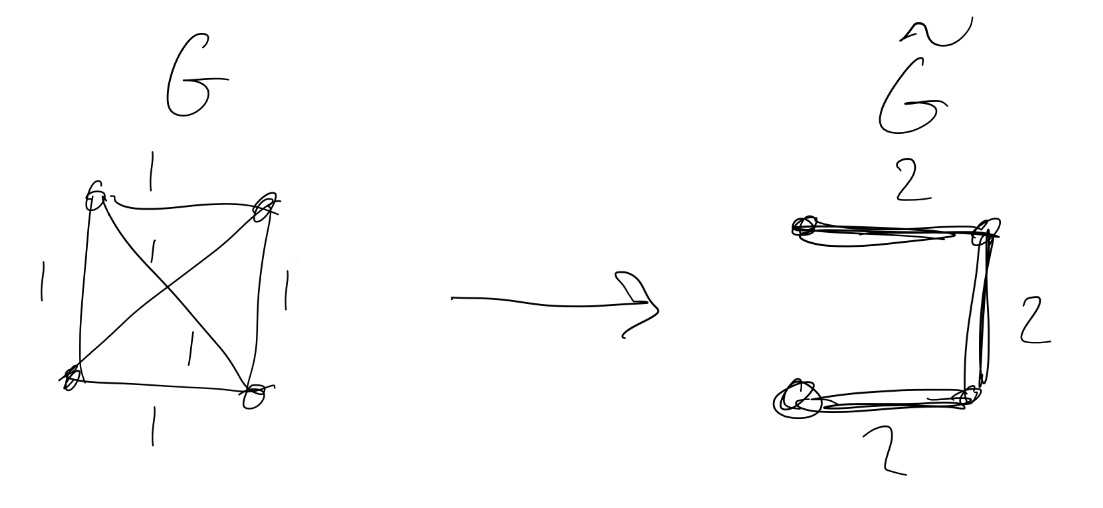
\includegraphics[width=0.6
  \textwidth]{fig/lecture8_gtil}
\caption{A graph $G$ and a spectral sparsifier $\Gtil$
,
  satisfisying
 $\LL_{G} \approx_{\epsilon} \LL_{\Gtil}$ for $\epsilon = 2.42$.
}
\label{fig:gvsgtil}
\end{figure}

We are going to construct $\Gtil$ by sampling some of the edges of $G$
according to a suitable probability distribution and scaling up their weight
to make up for the fact that we pick fewer of them.

To get a better understanding for the notion of approximation given in
\ref{def:psdapxeq} means, let's observe a simple consequence of it.

Given a vertex subset $T \subseteq V$, we say that $(T, V\setminus T)$
is a \emph{cut} in $G$ and that the value of the cut is
\[
  c_G(T) = \sum_{e \in E \intersect (T \times V\setminus T) } \ww(e)
.
\]

Figure~\ref{fig:cutexample} shows the $c_G(T)$ in a graph $G$.
\begin{figure}[h]
  \centering
  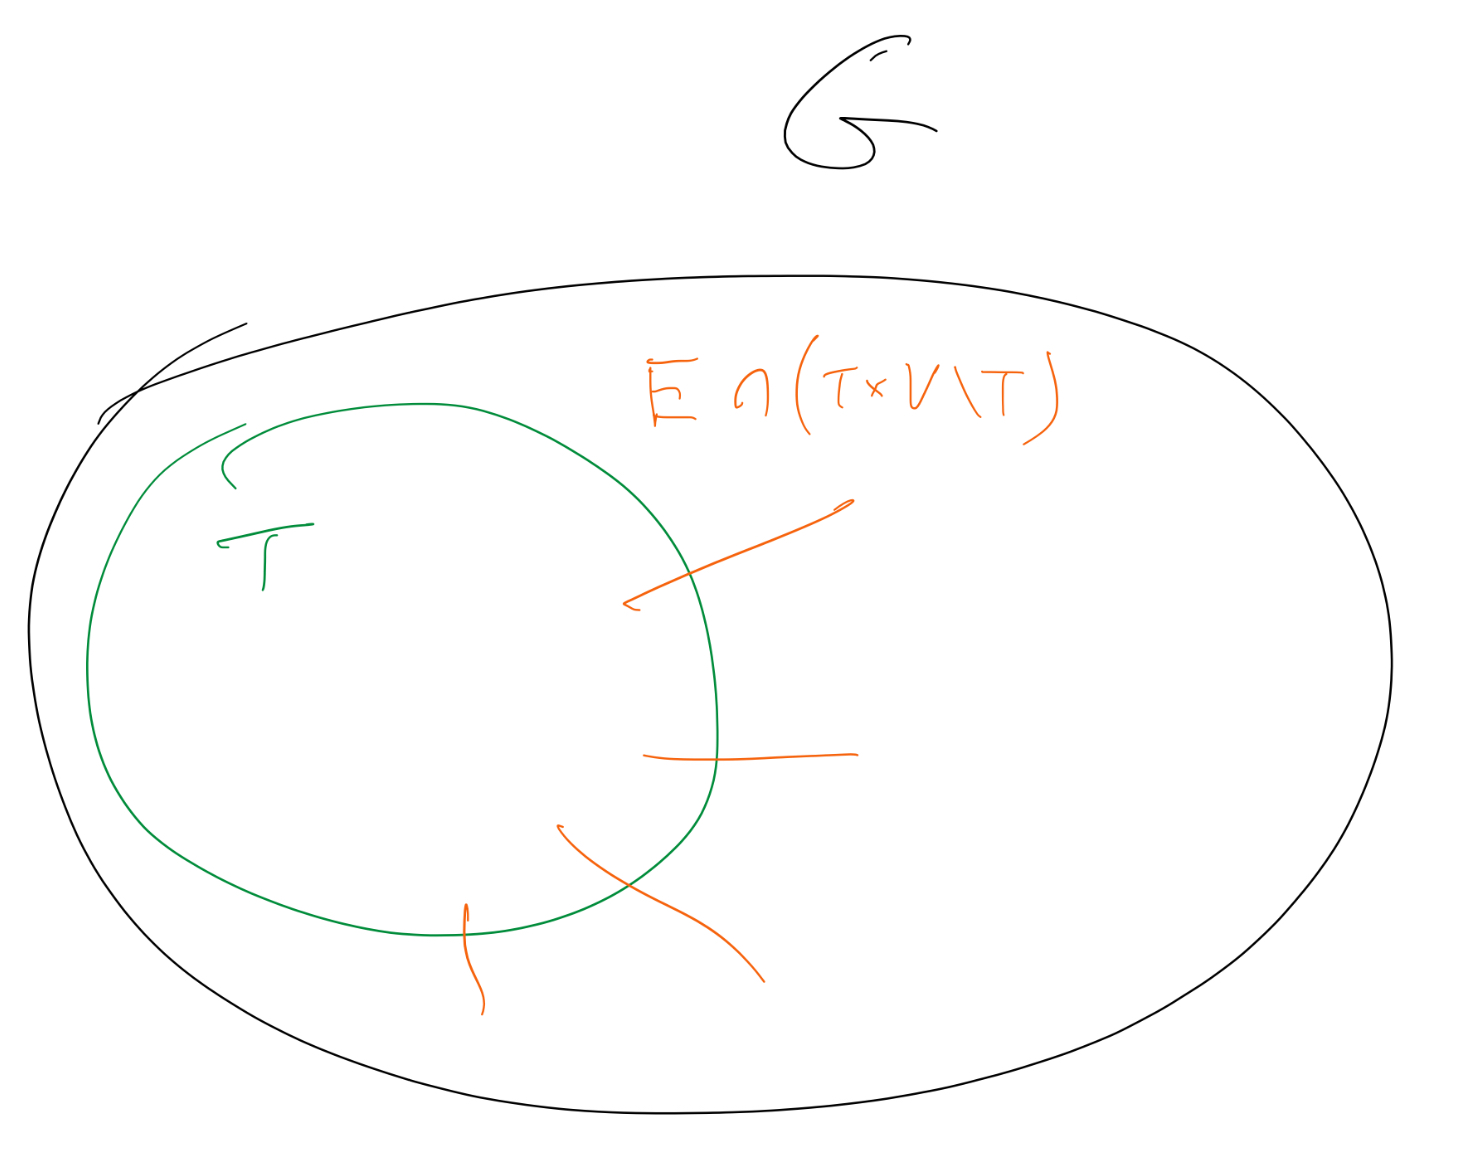
\includegraphics[width=0.4
  \textwidth]{fig/lecture8_cutvalue}
\caption{The cut $c_G(T)$ in $G$.}
\label{fig:cutexample}
\end{figure}


\begin{theorem}
  If $\LL_{G} \approx_{\epsilon} \LL_{\Gtil}$, then for all $T \subseteq V$,
  \[
    \frac{1}{1+\epsilon}   c_G(T) \leq   c_{\Gtil}(T) \leq (1+\epsilon)   c_G(T)
    .
    \]
\end{theorem}
\begin{proof}
  Let $\vecone_T \in \R^V$ be the indicator of the set $T$,
  i.e. $\vecone_T(u) = 1$ for $u \in V$ and $\vecone_T(u) = 0$
  otherwise.
  We can see that $\vecone_T^{\trp} \LL_{G} \vecone_T =  c_G(T)$, and
  hence the theorem follows by comparing the quadratic forms.
\end{proof}

But how well can we spectrally approximate a graph with a sparse graph? The next
theorem gives us a nearly optimal answer to this question.
\begin{theorem}[Spectral Graph Approximation by Sampling,
  (Spielman-Srivastava 2008)]
  \label{thm:spectralgraphapxbysamp}
Consider a connected graph $G = (V,E,\ww)$, with $n = \abs{V}$.
For any $0 < \epsilon < 1$
and $0 < \delta < 1$, there exist sampling probabilities $p_e$ for
each edge $e \in E$ s.t. if we include each edge $e$ in $\Etil$
independently with probabilty $p_e$ and set its weight $\wwtil(e) =
\frac{1}{p_e} \ww(e)$, then with probability at least $1-\delta$
the graph $\Gtil = (V,\Etil,\wwtil)$ satisfies
\[
  \LL_{G} \approx_{\epsilon} \LL_{\Gtil} \text{ and }  \abs{\Etil}
  \leq O( n \epsilon^{-2} \log(n/\delta) )
.
\]
\end{theorem}
The original proof can be found in \cite{spielman2011graph}.


\begin{remark}
  For convenience, we will abbreviate $\LL_{G}$ as $\LL$ and
  $\LL_{\Gtil}$ as $\LLtil$ in the rest of this section.
\end{remark}


We are going to analyze a sampling procedure by turning our goal into
a problem of matrix concentration.
Recall that
\begin{fact}
  $\AA \preceq \BB$ implies $\CC \AA \CC^\trp \preceq \CC \BB \CC^\trp
  $ for any $\CC \in \R^{n\times n}$.
\end{fact}
By letting $\CC = \LL^{\pinv/2}$, we can see that
\begin{equation}
  \label{eq:spectralreltoabs}
  \LL \approx_{\epsilon} \LLtil \text{ implies } \PPi_{\LL}
  \approx_{\epsilon} \LL^{\pinv/2}\LLtil\LL^{\pinv/2}
  ,
\end{equation}
where $\PPi_{\LL} = \LL^{\pinv/2}\LL\LL^{\pinv/2}$ is the orthogonal
projection to the complement of the kernel of $\LL$.
\begin{definition}
  Given a matrix $\AA$, we define $\PPi_{\AA}$ to be the orthogonal
  projection to the complement of the kernel of $\AA$,
  i.e. $\PPi_{\AA} \vv = \veczero$ for $\vv \in \ker(\AA)$ and
  $\PPi_{\AA} \vv = \vv$ for $\vv \in  \ker(\AA)^{\perp}$.
  Recall that $\ker(\AA)^{\perp} = \im(\AA^{\trp})$.
\end{definition}
\begin{claim}
  For a matrix $\AA \in \symsetn$ with spectral decomposition  $\AA =
  \VV\LLambda\VV^\trp = \sum_{i} \lambda_i \vv_i \vv_i^{\trp}$ s.t. $\VV^\trp \VV = \II$,
  we have $\PPi_{\AA} = \sum_{i : \lambda_i \neq 0} \vv_i \vv_i^{\trp}$, and
  $\PPi_{\AA} = \AA^{\pinv/2}\AA\AA^{\pinv/2} = \AA\AA^{\pinv} =  \AA^{\pinv}\AA $.
\end{claim}
From the definition, we can see that
$\PPi_{\LL}= \II - \frac{1}{n}\vecone\vecone^{\trp}$.

Now that we understand the projection $\PPi_{\LL}$, it is not hard to
show the following claim.
\begin{claim}
  \label{clm:spectralreltoabs}
  \noindent
\begin{enumerate}
\item
\label{enu:switchapxnormalizer}
  $\PPi_{\LL} \approx_{\epsilon} \LL^{\pinv/2}\LLtil\LL^{\pinv/2}$
  implies $\LL \approx_{\epsilon} \LLtil$.
\item
  \label{enu:normtoapx}
  For $\epsilon \leq 1$, we have that
  $\norm{\PPi_{\LL} - \LL^{\pinv/2}\LLtil\LL^{\pinv/2}} \leq
  \epsilon/2$ implies  $\PPi_{\LL} \approx_{\epsilon} \LL^{\pinv/2}\LLtil\LL^{\pinv/2}$.
\end{enumerate}
\end{claim}
Really, the only idea needed here is that when comparing quadratic
forms in matrices with
the same kernel, we necessarily can't have the quadratic forms
disagree on vectors in the kernel.
Simple! But we are going to write it out carefully, since we're still
getting used to these types of calculations.
\begin{proof}[Proof of Claim~\ref{clm:spectralreltoabs}]
  To prove Part~\ref{enu:normtoapx}, we
  assume $\PPi_{\LL} \approx_{\epsilon}
  \LL^{\pinv/2}\LLtil\LL^{\pinv/2}$.
  Recall that $G$ is a connected graph, so $\ker(\LL) =
  \Span\setof{\vecone}$, while $\LLtil$ is the Laplacian of a graph
which may or may not be connected, so $\ker(\LLtil) \supseteq
\ker(\LL)$, and equivalently $\im(\LLtil) \subseteq \im(\LL)$.
  Now, for any $\vv \in \ker(\LL)$ we have
  $\vv^{\trp} \LLtil \vv = 0 = \vv^{\trp} \LL \vv$.
  For any $\vv \in \ker(\LL)^{\perp}$ we have
  $\vv = \LL^{\pinv/2} \zz$ for some $\zz$, as $\ker(\LL)^{\perp} =
  \im(\LL) = \im(\LL^{\pinv/2})$.
  Hence
  \[
    \vv^{\trp} \LLtil \vv =
    \zz^{\trp} \LL^{\pinv/2}\LLtil\LL^{\pinv/2} \zz
    \geq
    \frac{1}{1+\epsilon}
     \zz^{\trp} \LL^{\pinv/2}\LL\LL^{\pinv/2} \zz
     =
     \frac{1}{1+\epsilon}
     \vv^{\trp} \LL \vv
   \]
and similarly
    \[
    \vv^{\trp} \LLtil \vv =
    \zz^{\trp} \LL^{\pinv/2}\LLtil\LL^{\pinv/2} \zz
    \leq
    (1+\epsilon)
     \zz^{\trp} \LL^{\pinv/2}\LL\LL^{\pinv/2} \zz
     =
    (1+\epsilon)
    \vv^{\trp} \LL \vv
    .
  \]
  Thus we have established  $\LL \approx_{\epsilon} \LLtil$.



  To prove Part~\ref{enu:normtoapx}, we assume $\norm{\PPi_{\LL} - \LL^{\pinv/2}\LLtil\LL^{\pinv/2}} \leq
  \epsilon/2$.
  This is equivalent to
  \[
   - \frac{\epsilon}{2} \II \preceq
    \LL^{\pinv/2}\LLtil\LL^{\pinv/2} - \PPi_{\LL} \preceq \frac{\epsilon}{2} \II
    \]
 But since
  \[
    \vecone^{\trp} (\LL^{\pinv/2}\LLtil\LL^{\pinv/2} - \PPi_{\LL})
    \vecone = 0,
  \]
  we can in fact sharpen this to
    \[
      - \frac{\epsilon}{2} \PPi_{\LL}
      \preceq
      \LL^{\pinv/2}\LLtil\LL^{\pinv/2} - \PPi_{\LL}
      \preceq
    \frac{\epsilon}{2} \PPi_{\LL}
    .
    \]
 Rearranging, we then conclude
 \[
   (1-\frac{\epsilon}{2}) \PPi_{\LL}
   \preceq
   \LL^{\pinv/2}\LLtil\LL^{\pinv/2}
    \preceq
    (1+\frac{\epsilon}{2}) \PPi_{\LL}
    .
  \]
Finally, we note that $1/(1+\epsilon) \leq (1-\frac{\epsilon}{2})$ to
reach our conclusion, $\PPi_{\LL} \approx_{\epsilon} \LL^{\pinv/2}\LLtil\LL^{\pinv/2}$.
\end{proof}

We now have most of the tools to prove
Theorem~\ref{thm:spectralgraphapxbysamp}, but to help us, we are going
to establish one small piece of helpful notation:
We define a matrix function $\Phi : \R^{n\times n} \to
\R^{n\times n} $
by
\[
  \Phi(\AA) = \LL^{\pinv/2}\AA\LL^{\pinv/2}.
  \]
We sometimes call this a ``normalizing map'', because it transforms a matrix to
the space where spectral norm bounds can be translated into relative
error guarantees compare to the $\LL$ quadratic form.
\begin{proof}[Proof of Theorem~\ref{thm:spectralgraphapxbysamp}]
  By Claim~\ref{clm:spectralreltoabs}, it suffices to show
  \begin{equation}
    \label{eq:spectralnormerrbound}
  \norm{\PPi_{\LL} - \LL^{\pinv/2}\LLtil\LL^{\pinv/2}} \leq
  \epsilon/2.
\end{equation}
  We introduce a set of independent random variables, one for each
  edge $e$, with a probability $p_e$ associated with the edge which we
  will fix later.
 We then let
  \[
    \YY_e =
    \begin{cases}
      \frac{\ww(e)}{p_e} \bb_e \bb_e^{\trp}
      & \text{ with probability } p_e
      \\
      \matzero
      & \text{ otherwise. }
    \end{cases}
  \]

This way, $\LLtil = \sum_e \YY_e$.
Note that $\E{\YY_e} = p_e \frac{\ww(e)}{p_e} \bb_e \bb_e^{\trp} =
\ww(e) \bb_e \bb_e^{\trp}$, and so
\[
  \E{\LLtil} =\sum_e \E{\YY_e} = \LL
  .
\]
By linearity of $\Phi$,
\[
\E{\Phi(\LLtil)} =  \Phi(\E{\LLtil}) = \PPi_{\LL}.
\]
Let us also define
\[
  \XX_e = \Phi(\YY_e) - \E {\Phi(\YY_e)} \text{ and } \XX = \sum_e \XX_e
\]
Note that this ensures $\E {\XX_e} = \matzero$.
We are now going to fix the edge sampling probabilities, in a way that
depends on some overall scaling parameter $\alpha > 0$.
We let
\[
  p_e = \min\left( \alpha \norm{\Phi\left(\ww(e)
      \bb_e\bb_e^{\trp} \right)}, 1 \right)
\]
then we see from the definition of $\YY_e$ that whenever $p_e < 1$
\[
  \norm{\Phi(\YY_e) } \leq \frac{1}{\alpha}
\]
from this, we can conclude, with a bit of work, that for all $e$
\begin{equation}
  \label{eq:bernsteinelementnormbound}
  \norm{\XX_e} \leq \frac{1}{\alpha}.
\end{equation}
We can also show that
\begin{equation}
  \label{eq:bernsteinvarnormbound}
  \norm{\sum_e \E{\XX_e^2}} \leq \frac{1}{\alpha}
  .
\end{equation}
In the exercises for this chapter, we will ask you to show that
Equations~\eqref{eq:bernsteinelementnormbound} and~\eqref{eq:bernsteinvarnormbound} holds.

This means that we can apply Theorem~\ref{thm:matbernstein} to our
$\XX = \sum_e \XX_e$, with $R =  \frac{1}{\alpha}$ and $\sigma^2 =
\frac{1}{\alpha}$, to get
\[
  \Pr\left[\norm{\PPi_{\LL} - \LL^{\pinv/2}\LLtil\LL^{\pinv/2}}
  \geq  \epsilon/2\right]
  \leq 2n\exp\left(\frac{-0.25 \epsilon^2}{(\epsilon +
      4)/\alpha}\right)
\]
Since $0 < \epsilon < 1$, this means that if
$\alpha = 40 \epsilon^{-2}  \log(n/\delta)$,
then
\[
  Pr\left[\norm{\PPi_{\LL} - \LL^{\pinv/2}\LLtil\LL^{\pinv/2}}
    \geq  \epsilon/2\right]
\leq \frac{2n\delta^2}{n^2} \leq \delta/2.
\]
In the last step, we assumed $n \geq 4$.

Lastly, we'd like to know that the graph $\Gtil$ is sparse.
The number of edges in $\Gtil$ is equal to the number of $\YY_e$ that
come out nonzero.
Thus, the expected value of $\abs{\Etil}$ is
\[
  \E{\abs{\Etil}}
  =
  \sum_e p_e \leq \alpha \sum_e \ww(e) \norm{\LL^{\pinv/2}\bb_e\bb_e^{\trp}\LL^{\pinv/2}}
\]
We can bound the sum of the norms with a neat trick relating it to the
trace of $\PPi_{\LL}$.
Note that in general for a vector $\aa \in \R^n$, we have
$\norm{\aa\aa^{\trp}} = \aa^{\trp}\aa = \trace{\aa\aa^{\trp}}$.
And hence
\begin{align*}
  \sum_e
  \ww(e)
  \norm{\LL^{\pinv/2}\bb_e\bb_e^{\trp}\LL^{\pinv/2}}
  &=
  \sum_e
  \ww(e)
  \trace{\LL^{\pinv/2}\bb_e\bb_e^{\trp}\LL^{\pinv/2}}
  \\
  &=
  \trace{ \LL^{\pinv/2}  \left( \sum_e\ww(e) \bb_e\bb_e^{\trp}
    \right)\LL^{\pinv/2}}
  \\
  &= \trace{ \PPi_{\LL} } = n-1.
\end{align*}
Thus with our choice of $\alpha$,
\[
  \E{\abs{\Etil}} \leq 40 \epsilon^{-2}  \log(n/\delta) n.
\]
With a scalar Chernoff bound, can show that $\abs{\Etil} \leq O( \epsilon^{-2}  \log(n/\delta) n)$
with probability at least $1-\delta/2$.
Thus by a union bound, the this condition and
Equation~\eqref{eq:spectralnormerrbound} are both satisfied with
probability at least $1-\delta$.
\end{proof}

\begin{remark}
  Note that
  \[
    \norm{\Phi\left(\ww(e) \bb_e\bb_e^{\trp} \right)}
    =
    \ww(e)
   \norm{\LL^{\pinv/2}\bb_e\bb_e^{\trp}\LL^{\pinv/2}}
  \leq
  \ww(e)\norm{ \LL^{\pinv/2}\bb_e}_2^2.
  \]
  Recall that in Chapter~\ref{cha:pinver}, we saw that the effective between vertex
  $v$ and vertex $u$ is given by
  $\norm{ \LL^{\pinv/2}(\ee_u - \ee_v)}_2^2$, and for an edge $e$
  connecting vertex $u$ and $v$, we have $\bb_{e}= \ee_u - \ee_v$.
 That means the norm of the ``baby Laplacian'' $\ww(e) \bb_e\bb_e^{\trp}$ of a single edge with weight
  $\ww(e)$ is exactly $\ww(e)$ times the effective resistance between
  the two endpoints of the edge.
\end{remark}

We haven't shown how to compute the sampling probabilities
efficiently, so right now, it isn't clear whether we can efficiently
find $\Gtil$.
It turns out that if we have access to a fast algorithm for solving
Laplacian linear equations, then we can find sufficiently good
approximations to the effective resistances quickly, and use these to
compute $\Gtil$.
An algorithm for this is described in \cite{spielman2011graph}.




\FloatBarrier


%%% Local Variables:
%%% mode: latex
%%% TeX-master: "agao21_script"
%%% TeX-engine: luatex
%%% End:
